% Final report in the course template (report/project_template.pdf). The submitted version is the Word file built by scripts/report_template_build.js (D-080); keep the text of both in step.
% Build:  tectonic main.tex     (or upload this folder to Overleaf; pdfLaTeX)
% Every number comes from report/numbers.json (scripts/report_numbers.py) or the Result files it cites.
\documentclass[11pt,a4paper]{article}

% ---------------------------------------------------------------- details to fill in
\newcommand{\University}{NED University of Engineering \& Technology}
\newcommand{\Department}{Department of Computer and Information Systems Engineering (CIS)}
\newcommand{\ProjectTitle}{Cost-Bounded Natural-Language Forensic Search over Surveillance Video}
\newcommand{\StudentName}{Wajahat Ahmed}
\newcommand{\StudentID}{CS-141/2026}
\newcommand{\Supervisor}{Dr Sharaf Hussain}
\newcommand{\SubmissionDate}{[Submission Date]}
\newcommand{\CodeLink}{[Google Drive link to the code and models]}

% ---------------------------------------------------------------- packages
\usepackage[T1]{fontenc}
\usepackage{lmodern}
\usepackage[a4paper,margin=2.5cm,headheight=14pt]{geometry}
\usepackage{amsmath,amssymb}
\usepackage{graphicx}
\usepackage{booktabs}
\usepackage{multirow}
\usepackage{array}
\usepackage{float}
\usepackage[font=normalsize,skip=6pt]{caption}
\usepackage{enumitem}
\usepackage{xcolor}
\usepackage{fancyhdr}
\usepackage{algorithm}
\usepackage{algpseudocode}
\usepackage{listings}
\usepackage{tikz}
\usetikzlibrary{arrows.meta,positioning,fit,backgrounds,calc}
\usepackage[colorlinks=true,linkcolor=blue,citecolor=blue,urlcolor=blue]{hyperref}

\graphicspath{{../figures/}}
\setlist{itemsep=2pt,topsep=4pt}

\pagestyle{fancy}
\fancyhf{}
\fancyhead[L]{Deep Learning Project Report}
\fancyhead[R]{\leftmark}
\fancyfoot[C]{\thepage}
\renewcommand{\headrulewidth}{0.4pt}

\definecolor{codebg}{RGB}{242,240,234}
\lstset{language=Python, basicstyle=\ttfamily\footnotesize, backgroundcolor=\color{codebg},
  keywordstyle=\color{magenta}, commentstyle=\color{gray}, stringstyle=\color{teal},
  numbers=left, numberstyle=\tiny\color{gray}, frame=single, rulecolor=\color{black!60},
  breaklines=true, columns=fullflexible, showstringspaces=false, xleftmargin=1.5em, framexleftmargin=1.5em}

\newcommand{\act}[1]{\textit{#1}}

\begin{document}

% ================================================================ title page
\begin{titlepage}
\centering
\vspace*{2.5cm}
{\Large \University\par}
\vspace{0.4cm}
{\large \Department\par}
\vspace{2.5cm}
\rule{\linewidth}{1.2pt}\par\vspace{0.4cm}
{\LARGE\bfseries \ProjectTitle\par}
\vspace{0.3cm}\rule{\linewidth}{1.2pt}\par
\vspace{1.5cm}
{\Large\itshape A Deep Learning Project Report\par}
\vspace{1.8cm}
{\bfseries Submitted by:\par}\vspace{0.2cm}
\StudentName \quad (\StudentID)\par
\vspace{0.6cm}
{\bfseries Supervised by:\par}\vspace{0.2cm}
\Supervisor\par
\vspace{0.6cm}
{\bfseries Course:\par}\vspace{0.2cm}
CS-5138 Deep Learning (Graduate)\par
\vfill
\SubmissionDate\par
\end{titlepage}

% ================================================================ front matter
\pagenumbering{roman}
\setcounter{page}{1}

\begin{center}\textbf{Abstract}\end{center}
\begin{quote}
This report presents \emph{\ProjectTitle}: searching surveillance activity clips with a typed sentence (``a
person opening a car door'') while making as few calls as possible to an expensive vision-language model (VLM).
We use MEVA, a public multi-camera surveillance dataset, from which 10,678 annotated activity clips were
downloaded, and a frozen test set of 66 queries over 22 activity types. Two protocols are evaluated: the official
split, and a split whose eight test cameras never appear in training. The system has three stages. The SigLIP~2
image encoder is adapted to the surveillance domain with LoRA (1.18\,M trained weights). A small temporal
transformer (2.2\,M weights) then re-ranks each clip from its frame embeddings and actor-box motion. An optional
VLM checks only the top ten clips. Seven VLMs (2B to 32B parameters) were tested as rankers. With no VLM calls,
category-search mAP rises from 0.179 (frozen encoder) to 0.313 with LoRA and 0.476 with the temporal
transformer; forensic Success@1 rises from 0.27 to 0.53, with similar gains on unseen cameras. A 2B VLM applied
to every clip scores below the cheap stages, distilling VLM scores into the student never beat training on the
human labels, and an 8B or 32B VLM on the top ten adds a further $+0.06$ Success@1. The pipeline runs as a
dashboard that turns any video into searchable alerts and reports the cost of each query.
\end{quote}

\vspace{0.5cm}
\noindent\textbf{Keywords:} deep learning, text-to-video retrieval, vision-language models, LoRA, temporal
transformer, surveillance video, cost-aware re-ranking

\clearpage
\tableofcontents
\clearpage
\listoffigures
\listoftables
\clearpage

\pagenumbering{arabic}
\setcounter{page}{1}

% ================================================================ 1
\section{Introduction}

\subsection{Background and Motivation}
A surveillance installation produces hours of footage and thousands of automated alerts every day. When an
incident is reported after the fact, investigators scrub that footage by camera and time, because nothing indexes
what the footage \emph{shows}. Natural-language search would let an investigator type ``a person taking a bag
from a parked car'' and receive the matching clips. Vision-language models (VLMs) can judge such a query well:
shown a clip, they answer ``does this show \ldots?''. But one VLM call per clip is slow, and over an archive it
costs minutes per query (about 10 minutes for 3,726 clips with a 2B model on a laptop GPU) and real money with a
paid API. The practical question is therefore not only how accurate the search is, but how much accuracy is
kept as the number of expensive calls is cut.

\subsection{Problem Statement}
\textbf{Input:} a free-text query $q$ and a corpus of surveillance clips $\mathcal{C}$, each an annotated activity
instance (actors' boxes, start and end time), optionally restricted to a camera and hour.
\textbf{Output:} a ranking of $\mathcal{C}$ by relevance to $q$.
\textbf{Objective:} maximise retrieval quality (mAP, Success@$K$) under a budget of VLM calls per query, and
measure the whole quality-versus-cost curve: how much of the accuracy of a VLM applied to every clip can be kept
with one to two orders of magnitude fewer calls?

\subsection{Objectives}
\begin{itemize}
  \item \textbf{Objective 1:} build a retrieval benchmark on MEVA, a public surveillance dataset that had never
        been used for natural-language retrieval: a frozen query set and two evaluation protocols.
  \item \textbf{Objective 2:} adapt a pretrained image--text encoder (SigLIP~2) to fixed surveillance cameras with
        LoRA, and measure the gain on seen and unseen cameras.
  \item \textbf{Objective 3:} add a cheap learned re-ranker and decide, with fixed gates, whether and where a VLM is
        worth its cost; report the quality-versus-cost curve.
  \item \textbf{Objective 4:} run the pipeline end to end on new video: detected alerts, searchable by text, with
        the cost of each query shown.
\end{itemize}

\subsection{Scope and Limitations}
\textbf{In scope:} retrieval of annotated activity instances (the unit an alert pipeline produces); 22 activity
types with at least 20 test instances; models that run on one 8\,GB laptop GPU, plus a 16\,GB office GPU for the
8B and 32B VLMs; cost counted as VLM calls and seconds.
\textbf{Out of scope:} finding the start and end of an event inside long untrimmed video; identifying people (the
system retrieves events, not persons, by design); paid APIs, so no token or money cost.
\textbf{Limitations:} MEVA activities are scripted by actors, so absolute numbers may be optimistic for
uncontrolled footage; each selected model was trained with one seed; and no labels exist for footage from outside
MEVA, so its retrieval quality is shown, not measured.

\subsection{Report Organization}
Section~\ref{sec:related} reviews related work. Section~\ref{sec:data} describes the dataset, preprocessing and the
two splitting protocols. Section~\ref{sec:method} presents the architecture, losses, optimisation and training
procedure. Section~\ref{sec:exp} reports the experiments: baselines, the main comparison, qualitative results and
ablations. Section~\ref{sec:disc} discusses the findings and Section~\ref{sec:concl} concludes. Appendix~\ref{app:code}
links the code and models and explains how to install and run the system; Appendix~\ref{app:more} holds
additional results.

% ================================================================ 2
\section{Related Work}\label{sec:related}

\paragraph{Contrastive image--text encoders.} CLIP~\cite{clip} trained an image and a text encoder jointly on 400
million web image--caption pairs, so that images can be classified and searched zero-shot from text, and so that
image embeddings can be computed once and indexed. SigLIP~\cite{siglip} replaced the batch-wide softmax with a
per-pair sigmoid loss that needs no global normalisation, and SigLIP~2~\cite{siglip2} added captioning-based
pretraining, self-distillation and data curation, improving zero-shot classification and retrieval at every model
size. This project uses SigLIP~2 ViT-B/16 as its retriever. All three are trained on web photographs, not fixed,
elevated cameras with small, distant people.

\paragraph{Video moment retrieval and its cost.} Escorcia et al.~\cite{escorcia} posed moment retrieval over a whole
video collection and showed that clip-level alignment allows the corpus to be indexed in advance.
QVHighlights~\cite{qvhighlights} released free-form queries on 10,000 YouTube videos. Tran et
al.~\cite{tran} combined coarse and fine encoders with temporal re-ranking for hour-long video, and Nishimura et
al.~\cite{superimage} screened candidates with a cheap model before a VLM, showing that the accuracy--cost
trade-off moves with model size and resolution; that is the closest precedent for our cascade. None of these
evaluates on surveillance footage.

\paragraph{Surveillance video and language.} UCA~\cite{uca} annotated 110 hours of UCF-Crime with sentences and found
that models strong on web video perform poorly on surveillance (fixed viewpoints, low resolution, small subjects).
VadCLIP~\cite{vadclip} adapted CLIP to anomaly detection, a closed set of classes. SurveiLens~\cite{surveilens}
captions sampled frames and matches the captions to a query; ForeSea~\cite{foresea} filters footage with a tracker,
indexes it with a multimodal embedding and answers with a video LLM over the top clips. Both report accuracy, not
the number of expensive calls per query.

\paragraph{Adaptation and distillation.} LoRA~\cite{lora} trains low-rank updates of frozen weight matrices, matching
full fine-tuning with far fewer trained parameters. Knowledge distillation~\cite{hinton} trains a small model on the
soft outputs of a large one, and Hofst\"atter et al.~\cite{hofstatter} distilled a cross-encoder ranker into cheaper
students. Cascade ranking~\cite{cascade} orders rankers by cost, each pruning candidates for the next.

\paragraph{How this work differs.} (1) The surveillance retrieval systems above report accuracy only; we report
accuracy \emph{as a function of VLM calls}. (2) MEVA~\cite{meva}, the largest annotated fixed-camera activity
corpus with a permissive licence, had not been used for natural-language retrieval. (3) We measure the web-to-CCTV
domain shift of a dual encoder on seen and unseen cameras, with and without adaptation. (4) We test the proposed
distillation route against a student trained on human labels, and report that it does not help.

% ================================================================ 3
\section{Dataset and Preprocessing}\label{sec:data}

\subsection{Dataset Description}
MEVA (Multiview Extended Video with Activities)~\cite{meva} was recorded by Kitware for the IARPA DIVA programme:
fixed indoor and outdoor cameras at a training facility, actors performing scripted everyday activities, released
under CC BY 4.0 with human annotations (actor bounding boxes, activity labels, start and end times). It is public,
not hosted on Kaggle and not synthetic, and is available at \url{https://mevadata.org} (videos on AWS Open Data,
\url{https://registry.opendata.aws/mevadata/}). We downloaded the video of 10,678 annotated activity instances (about
70\,GB): 32 activity types, 24 cameras at 4 sites. The 22 types with at least 20 test instances are the query
activities; the 10 rarer types stay in the corpus as distractors. The distribution is long-tailed (447 instances
of \act{enters scene through structure} against 21 of \act{vehicle reverses} in the test split of protocol A).

There were no text queries, so we wrote them: 3 natural phrasings per query activity (66 in total), drafted from
MEVA's activity definitions, reviewed on training-split examples, and frozen by hash before the first evaluation.
A separate bank of 192 training captions is used for fine-tuning; it shares no sentence with the test phrasings,
and same-activity caption--phrasing similarity is below 0.80.

\begin{table}[H]
\centering
\caption[Summary of the dataset used in this project.]{Summary of the dataset used in this project (instances = clips).}\label{tab:data}
\small
\begin{tabular}{llrrl}
\toprule
\textbf{Protocol} & \textbf{Split} & \textbf{\# Samples} & \textbf{\# Classes} & \textbf{Notes} \\
\midrule
\multirow{3}{*}{A (official)} & Training   & 6,213 & 32 & 192 training captions \\
                              & Validation &   739 & 15 & model selection only \\
                              & Test       & 3,726 & 32 & 22 query activities, 66 phrasings \\
\midrule
\multirow{3}{*}{B (unseen cameras)} & Training   & 6,154 & 32 & 16 cameras \\
                                    & Validation &   586 & 15 & same 16 cameras \\
                                    & Test       & 3,938 & 32 & 8 cameras never seen in training \\
\midrule
\multicolumn{2}{l}{Total} & 10,678 & 32 & 24 cameras, 4 sites \\
\bottomrule
\end{tabular}
\end{table}

\subsection{Preprocessing}
\begin{itemize}
  \item \textbf{Frame sampling:} each instance is sampled at 2 frames per second, at most 16 frames.
  \item \textbf{Crops:} from the annotated actor boxes, each frame gets a square \emph{tight} crop around the actors at
        native resolution, and a \emph{context} crop with surroundings ($\le$448\,px). On validation, tight crops
        doubled top-10 precision over full frames (0.22 against 0.10), so the tight view was fixed before any test
        number was read.
  \item \textbf{Image normalisation:} crops are resized to $224\times224$ (bilinear) and normalised exactly as the
        SigLIP~2 processor does; the training pipeline reproduces the processor pixel-for-pixel (tested).
  \item \textbf{Augmentation (LoRA training only):} zoom in/out, stretch and resolution degradation. No horizontal
        flips, because left and right turns are different activities.
  \item \textbf{Text:} SigLIP~2 tokenizer, padded to 64 tokens, as in its pretraining.
  \item \textbf{Box motion:} per frame, 12 numbers from the actor boxes (cumulative and per-step displacement, log
        height and width, aspect ratio, number of actors, distance between actors, time, a has-box flag).
  \item \textbf{Class balance:} square-root-balanced sampling of instances during fine-tuning, and every metric is
        macro-averaged over the 22 activities so frequent classes cannot hide rare-class failures.
\end{itemize}

\subsection{Data Splitting Strategy}
Two protocols are evaluated. \textbf{Protocol A} is MEVA's official split; its test cameras also appear in
training. \textbf{Protocol B} holds 8 of the 24 cameras out of training and validation entirely, so the gap between
A and B measures how much a model relies on having seen a camera. In both, the split is by recording, not by
frame, so no clip contributes frames to two splits. \textbf{Selection rule:} every model, epoch, weight and
threshold was chosen on the validation split; the test split was read once per result and never used to choose
anything.

% ================================================================ 4
\section{Methodology}\label{sec:method}

\subsection{Proposed Architecture}
Figure~\ref{fig:arch} shows the system. At index time every clip is embedded once; at query time a sentence costs
one text-encoder call, a dot product with every frame, and a pass of the small transformer over the candidates.

\begin{figure}[H]
\centering
\resizebox{\linewidth}{!}{%
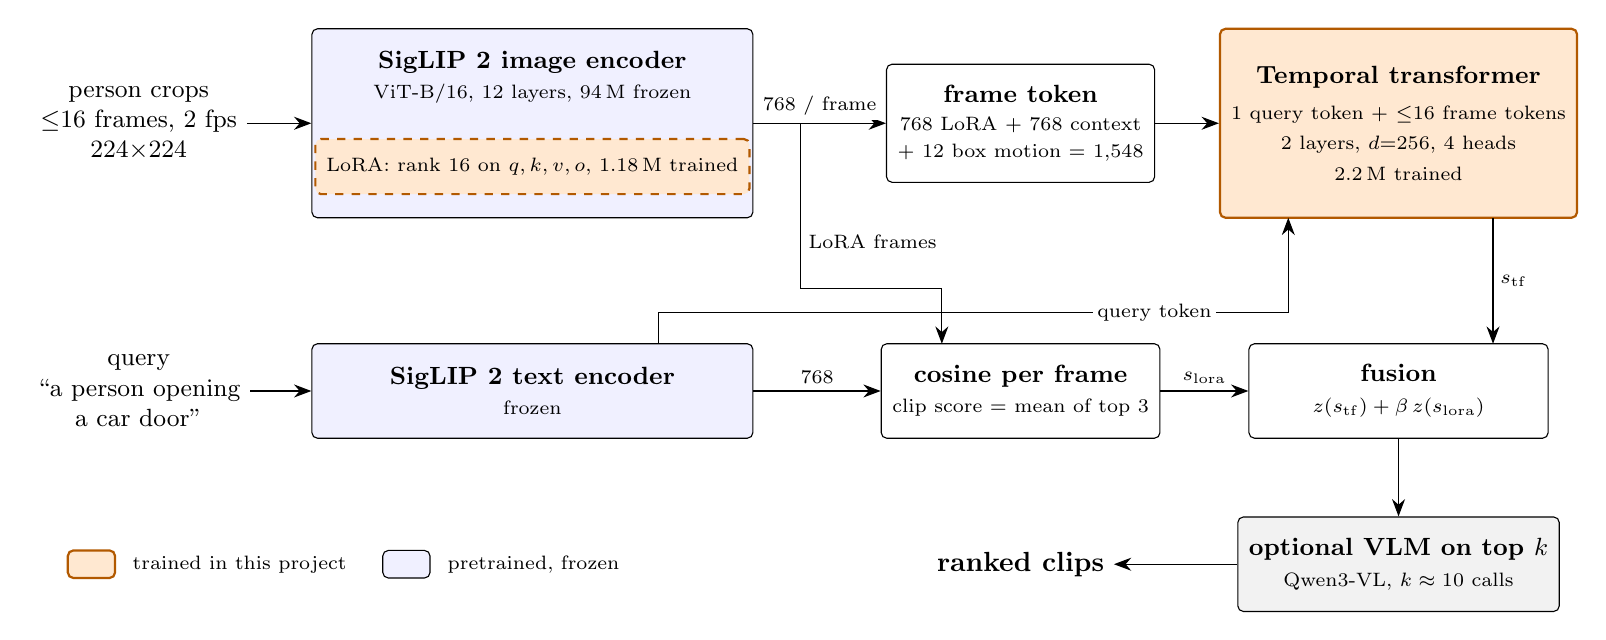
\begin{tikzpicture}[
  font=\small, >={Stealth[length=2.2mm]},
  box/.style={draw, rounded corners=2pt, align=center, inner sep=4pt},
  frozen/.style={box, fill=blue!6},
  trained/.style={box, fill=orange!18, draw=orange!70!black, thick},
  lab/.style={font=\scriptsize, align=center, fill=white, inner sep=1.5pt}]
% ---- row 1: image path
\node[align=center] (crops) at (0,0) {person crops\\$\le$16 frames, 2 fps\\$224{\times}224$};
\node[frozen, minimum width=5.6cm, minimum height=2.4cm] (enc) at (5.0,0) {};
\node[font=\small\bfseries] at (5.0,0.78) {SigLIP 2 image encoder};
\node[font=\scriptsize] at (5.0,0.38) {ViT-B/16, 12 layers, 94\,M frozen};
\node[trained, dashed, minimum width=4.9cm, minimum height=0.7cm, font=\scriptsize] (lora) at (5.0,-0.55)
  {LoRA: rank 16 on $q,k,v,o$, 1.18\,M trained};
\node[box, minimum width=2.9cm, minimum height=1.5cm] (tok) at (11.2,0)
  {\textbf{frame token}\\[-1pt]{\scriptsize 768 LoRA + 768 context}\\[-1pt]{\scriptsize + 12 box motion = 1,548}};
\node[trained, minimum width=3.8cm, minimum height=2.4cm] (tf) at (16.0,0)
  {\textbf{Temporal transformer}\\[2pt]{\scriptsize 1 query token + $\le$16 frame tokens}\\{\scriptsize 2 layers, $d{=}256$, 4 heads}\\{\scriptsize 2.2\,M trained}};
% ---- row 2: text path
\node[align=center] (q) at (0,-3.4) {query\\``a person opening\\a car door''};
\node[frozen, minimum width=5.6cm, minimum height=1.2cm] (tenc) at (5.0,-3.4) {\textbf{SigLIP 2 text encoder}\\{\scriptsize frozen}};
\node[box, minimum width=2.9cm, minimum height=1.2cm] (cos) at (11.2,-3.4) {\textbf{cosine per frame}\\{\scriptsize clip score = mean of top 3}};
\node[box, minimum width=3.8cm, minimum height=1.2cm] (fuse) at (16.0,-3.4) {\textbf{fusion}\\{\scriptsize $z(s_{\mathrm{tf}}) + \beta\, z(s_{\mathrm{lora}})$}};
% ---- row 3: output
\node[box, fill=gray!10, minimum width=3.8cm, minimum height=1.2cm] (vlm) at (16.0,-5.6) {\textbf{optional VLM on top $k$}\\{\scriptsize Qwen3-VL, $k \approx 10$ calls}};
\node[font=\bfseries] (out) at (11.2,-5.6) {ranked clips};
% ---- arrows
\draw[->] (crops) -- (enc);
\draw[->] (enc) -- node[lab, above=1pt] {768 / frame} (tok);
\draw[->] (tok) -- (tf);
\draw[->] (q) -- (tenc);
\draw[->] (tenc) -- node[lab, above=1pt] {768} (cos);
\draw[->] (8.4,0) -- (8.4,-2.1) -| (10.2,-2.8);
\node[lab, anchor=west] at (8.45,-1.5) {LoRA frames};
\draw[->] (6.6,-2.8) -- (6.6,-2.4) -| (14.6,-1.2);
\node[lab] at (12.9,-2.4) {query token};
\draw[->] (cos) -- node[lab, above=1pt] {$s_{\mathrm{lora}}$} (fuse);
\draw[->] (17.2,-1.2) -- node[lab, right=1pt] {$s_{\mathrm{tf}}$} (17.2,-2.8);
\draw[->] (fuse) -- (vlm);
\draw[->] (vlm) -- (out);
% ---- legend
\node[trained, minimum width=0.6cm, minimum height=0.35cm] (lg1) at (-0.6,-5.6) {};
\node[anchor=west, font=\scriptsize] at (-0.2,-5.6) {trained in this project};
\node[frozen, minimum width=0.6cm, minimum height=0.35cm] (lg2) at (3.4,-5.6) {};
\node[anchor=west, font=\scriptsize] at (3.8,-5.6) {pretrained, frozen};
\end{tikzpicture}}
\caption[Overview of the proposed model architecture.]{Overview of the proposed model architecture. The three search levels of the dashboard are
\emph{Fast} (cosine score only), \emph{Standard} (fusion with the temporal transformer, the main system) and
\emph{Verified} (Standard, then the VLM on the top $k$).}\label{fig:arch}
\end{figure}

\paragraph{Stage 1: adapted retriever.} SigLIP~2 base (ViT-B/16, 224\,px)~\cite{siglip2} embeds every tight crop and
the query into the same 768-dimensional space; vectors are $\ell_2$-normalised, so the dot product is the cosine
similarity. A clip's score is the mean of its three highest frame similarities, which tolerates frames in which the
action has not started. LoRA~\cite{lora} adapters of rank 16 are added to the query, key, value and output
projections of all 12 attention layers of the image encoder (48 adapters, 1.18\,M trained weights, 1.25\,\% of
the encoder). The text encoder stays frozen, so query encoding and general language are unchanged.

\paragraph{Stage 2: temporal transformer (``student'').} A single frame cannot show standing up or picking something
up. The re-ranker reads one token per frame (1,548 numbers: the LoRA tight embedding, the frozen context embedding
and the 12 box-motion features) and one token for the query (768 numbers). Each token is layer-normalised and
projected to $d=256$; frames get a learned position embedding. A 2-layer pre-norm transformer encoder (4 heads,
feed-forward 1,024, dropout 0.1) processes the at most 17 tokens; the output at the query token goes through a
linear head to one relevance logit $s_{\mathrm{tf}}$. Its score is fused with the retriever's,
$s = z(s_{\mathrm{tf}}) + \beta\,z(s_{\mathrm{lora}})$, where $z$ standardises over the candidates and $\beta$
is chosen on validation ($\beta=1$).

\paragraph{Stage 3: VLM on a short list (optional).} A VLM scores a clip by the log-odds of ``yes'' over ``no'' to
``Does this video show the following: \{query\}?'', given 8 evenly spaced tight frames at 448\,px with their
timestamps. It re-orders only the top $k$ of stage 2 by $z(\mathrm{VLM}) + \gamma\, z(s)$ ($\gamma=2$, chosen on
validation). Two gates fixed in advance decide whether a VLM is used: G0 (fits in memory, deterministic) and G1
(adds at least $+0.02$ validation mAP when fused into the adapted retriever's top 50).

\subsection{Loss Function}
\paragraph{LoRA: label-aware sigmoid loss.} For a batch of $N$ crop embeddings $\mathbf{x}_i$ and $M$ caption
embeddings $\mathbf{t}_j$, with the pretrained temperature $\tau$ and bias $b$ of SigLIP (also trained),
\begin{equation}
\mathcal{L}_{\mathrm{LoRA}}(\theta) = -\frac{1}{N}\sum_{i=1}^{N}\sum_{j=1}^{M}
\Big[ y_{ij}\log\sigma(\ell_{ij}) + (1-y_{ij})\log\big(1-\sigma(\ell_{ij})\big) \Big],
\qquad \ell_{ij} = \tau\,\mathbf{x}_i^{\top}\mathbf{t}_j + b ,
\end{equation}
where $y_{ij}=1$ when caption $j$ describes the activity of crop $i$. It differs from SigLIP's loss in one point:
every caption of the crop's activity is a positive, not only its own caption.

\paragraph{Temporal transformer: binary cross-entropy.} For a (clip, caption) pair $p$ with logit $s_p$, label
$y_p\in\{0,1\}$ and, when a teacher is used, the teacher's VLM margin $m_p$,
\begin{equation}
\mathcal{L}_{\mathrm{tf}} = -\frac{1}{P}\sum_{p=1}^{P}\Big[\tilde y_p \log\sigma(s_p) + (1-\tilde y_p)\log\big(1-\sigma(s_p)\big)\Big],
\qquad \tilde y_p = \alpha\, y_p + (1-\alpha)\,\sigma(m_p) .
\end{equation}
$\alpha=1$ trains on the human labels (GT), $\alpha=0.5$ mixes in the teacher (GT+KD, the distillation route), and
$\alpha=0$ trains on the teacher alone (KD).

\subsection{Optimization}
Both trained components use AdamW. \textbf{LoRA:} learning rate $10^{-4}$, batch 64, linear warm-up over 2 epochs,
then the rate is halved after every 2 epochs without a validation gain; at most 100 epochs, early stopping after 5
epochs without a gain (best epochs 10--28; the cap was never reached). \textbf{Temporal transformer:} learning rate
$3\times10^{-4}$, batch 256, at most 50 epochs, early stopping after 5 epochs without a gain. The model of the
best validation epoch is kept. The validation metric is Q1 mAP on the validation split.

\subsection{Regularization and Hyperparameters}
\begin{table}[H]
\centering
\caption{Hyperparameter configuration.}\label{tab:hyper}
\small
\begin{tabular}{lll}
\toprule
\textbf{Hyperparameter} & \textbf{LoRA (image encoder)} & \textbf{Temporal transformer} \\
\midrule
Optimizer & AdamW & AdamW \\
Learning rate & $1\times10^{-4}$, warm-up 2 epochs & $3\times10^{-4}$ \\
LR schedule & $\times0.5$ after 2 epochs without gain & constant \\
Batch size & 64 crops & 256 pairs \\
Epochs & $\le100$, early stop patience 5 & $\le50$, early stop patience 5 \\
Weight decay & 0.01 (adapters only) & 0.01 \\
Dropout & 0.1 (LoRA dropout) & 0.1 \\
Size & rank 16, $\alpha=32$, 48 adapters, 1.18\,M & 2 layers, $d=256$, 4 heads, 2.2\,M \\
Training data & 6,213 instances $\times$ 192 captions & $\approx$12,200 pairs per protocol \\
Fusion weight & -- & $\beta=1$ (grid on validation) \\
\bottomrule
\end{tabular}
\end{table}

Other regularisation: square-root class balancing, crop augmentation (Section~\ref{sec:data}), a frozen text encoder,
and the restriction of LoRA to the attention projections. The rank, $\alpha$ and the transformer's size were fixed in
the plan before training and not tuned.

\subsection{Training Procedure}
Four LoRA runs were trained (protocol A or B $\times$ uniform or middle-weighted frame sampling) and one was
selected per protocol on validation. The training pairs of the temporal transformer are, for each activity, its
positive clips plus 100 hard negatives (the highest-scoring wrong clips under LoRA) and 100 random negatives.

\begin{algorithm}[H]
\caption{Training procedure (LoRA retriever, then temporal transformer)}\label{alg:train}
\begin{algorithmic}[1]
\Require training clips $\mathcal{D}_{\mathrm{train}}$, captions $\mathcal{T}$, validation set $\mathcal{D}_{\mathrm{val}}$
\State Load SigLIP 2; freeze all weights; insert LoRA adapters $\theta$ (rank 16) into the image encoder
\For{epoch $e = 1$ \textbf{to} 100}
  \For{each mini-batch $\mathcal{B}$ of crops (square-root class-balanced, augmented)}
    \State $\mathbf{x} \gets$ image encoder$_\theta(\mathcal{B})$;\ $\mathbf{t} \gets$ text encoder$(\mathcal{T})$
    \State compute $\mathcal{L}_{\mathrm{LoRA}}$ (Eq.~1);\ $\theta \gets \mathrm{AdamW}(\theta, \nabla_\theta \mathcal{L})$
  \EndFor
  \State evaluate validation Q1 mAP; keep the best $\theta$; halve the LR after 2 epochs, stop after 5, without gain
\EndFor
\State Re-embed every clip with the best adapters; build frame tokens (LoRA + context + box motion)
\State Build pairs: positives + 100 hard + 100 random negatives per activity
\For{epoch $e = 1$ \textbf{to} 50}
  \For{each mini-batch of 256 (clip, caption) pairs}
    \State $s \gets$ transformer$_\phi$(query token, frame tokens);\ $\phi \gets \mathrm{AdamW}(\phi, \nabla_\phi \mathcal{L}_{\mathrm{tf}})$ (Eq.~2)
  \EndFor
  \State choose $\beta$ on validation; keep the best $(\phi,\beta)$; stop after 5 epochs without gain
\EndFor
\State \Return adapters $\theta$, transformer $\phi$, fusion weight $\beta$
\end{algorithmic}
\end{algorithm}

% ================================================================ 5
\section{Experiments and Results}\label{sec:exp}

\subsection{Experimental Setup}
\textbf{Hardware:} a laptop with an NVIDIA RTX 4060 Laptop GPU (8\,GB) and 32\,GB RAM for everything except the 8B
and 32B VLMs, which ran on an office server with an RTX 4070 Ti SUPER (16\,GB; the 32B with weights streamed
between CPU and GPU). \textbf{Software:} Python 3.12, PyTorch 2.14 (CUDA 12.6), Hugging Face Transformers 5.20,
PEFT 0.21, Ultralytics YOLOv8 8.4. \textbf{Runtime:} one LoRA epoch takes about 57\,s; all four LoRA runs 1.5\,h;
a temporal transformer run a few minutes. At query time the Standard level takes about 0.26\,s for the 3,726 test
clips, of which the transformer is 0.18\,s. Appendix~\ref{app:code} explains how to install and run the
system.

\subsection{Evaluation Metrics}
Two query types are evaluated. \textbf{Q1, category search:} each of the 66 phrasings ranks the whole test corpus.
\textbf{Q2, forensic search:} ``find it on camera $C$ in hour $H$'', one query per annotated event and phrasing
(1,140 per protocol), ranked inside that camera-hour (median 56 candidates). For a ranking with relevant set $R$,
\begin{equation}
\mathrm{AP} = \frac{1}{|R|}\sum_{k=1}^{n} P@k \cdot \mathrm{rel}(k),\qquad
\mathrm{Success@}K = \mathbb{1}\!\left[\exists\, k \le K:\ \mathrm{rel}(k)=1\right],
\end{equation}
\begin{equation}
\mathrm{RR} = \frac{1}{\text{rank of the first relevant clip}}, \qquad \mathrm{MRR} = \text{mean of RR over queries},
\end{equation}
with $P@k$ the precision of the top $k$. mAP is the mean AP over queries; P@10 and Recall@10 are also reported.
All metrics are \emph{macro-averaged over the 22 activities}. 95\,\% confidence intervals come from a paired
bootstrap over activities (10,000 resamples). Cost is the number of VLM calls and the seconds per query.

\subsection{Quantitative Results}
\begin{table}[H]
\centering
\caption[Comparison of models on the test set.]{Comparison of models on the test set (Q1 = category search, Q2 = forensic search; VLM calls per Q2 query).}\label{tab:main}
\footnotesize
\setlength{\tabcolsep}{4pt}
\begin{tabular}{llrccccc}
\toprule
& & \textbf{VLM} & \multicolumn{2}{c}{\textbf{Q1}} & \multicolumn{3}{c}{\textbf{Q2}} \\
\cmidrule(lr){4-5}\cmidrule(lr){6-8}
\textbf{Prot.} & \textbf{Model} & \textbf{calls} & \textbf{mAP} & \textbf{P@10} & \textbf{S@1} & \textbf{S@5} & \textbf{MRR} \\
\midrule
A & Zero-shot CLIP ViT-B/16 (baseline) & 0 & 0.142 & 0.189 & 0.237 & 0.558 & 0.391 \\
A & Zero-shot SigLIP 2, full frame & 0 & 0.096 & 0.127 & -- & -- & 0.267 \\
A & Zero-shot SigLIP 2, tight crops & 0 & 0.179 & 0.259 & 0.273 & 0.655 & 0.447 \\
A & + LoRA & 0 & 0.313 & 0.408 & 0.389 & 0.797 & 0.558 \\
A & \textbf{+ LoRA + temporal transformer (proposed)} & \textbf{0} & \textbf{0.476} & \textbf{0.527} & \textbf{0.531} & \textbf{0.900} & \textbf{0.690} \\
A & \quad + 8B VLM on top 10 & 9.8 & 0.477 & 0.527 & 0.589 & 0.914 & 0.728 \\
A & \quad + 32B VLM on top 10 & 9.8 & 0.478 & 0.527 & 0.597 & 0.912 & 0.732 \\
A & 2B VLM on every candidate & 124.5 & 0.207 & 0.312 & 0.360 & 0.729 & 0.523 \\
\midrule
B & Zero-shot CLIP ViT-B/16 (baseline) & 0 & 0.138 & 0.192 & 0.261 & 0.584 & 0.409 \\
B & Zero-shot SigLIP 2, tight crops & 0 & 0.174 & 0.274 & 0.275 & 0.703 & 0.460 \\
B & + LoRA & 0 & 0.280 & 0.362 & 0.369 & 0.723 & 0.528 \\
B & \textbf{+ LoRA + temporal transformer (proposed)} & \textbf{0} & \textbf{0.442} & \textbf{0.521} & \textbf{0.519} & \textbf{0.848} & \textbf{0.663} \\
B & \quad + 8B VLM on top 10 & 9.7 & 0.443 & 0.521 & 0.554 & 0.859 & 0.692 \\
B & \quad + 32B VLM on top 10 & 9.7 & 0.444 & 0.521 & 0.564 & 0.867 & 0.692 \\
B & 2B VLM on every candidate & 307.8 & 0.212 & 0.312 & 0.367 & 0.729 & 0.531 \\
\bottomrule
\end{tabular}
\end{table}

Random ordering gives Q1 mAP 0.047. Every stage improves every metric on both protocols:
\begin{itemize}
  \item \textbf{LoRA:} Q1 mAP $+0.134$ [$+0.085$, $+0.194$] on A and $+0.107$ [$+0.062$, $+0.158$] on B; Q2 Success@1
        $+0.115$ and $+0.094$. About 80\,\% of the gain carries over to cameras never seen in training.
  \item \textbf{Temporal transformer:} Success@1 $+0.143$ [$+0.058$, $+0.228$] on A and $+0.150$ [$+0.082$, $+0.220$] on
        B, at zero VLM calls; Q1 mAP $+0.163$ and $+0.162$. This is the largest single step.
  \item \textbf{VLMs:} an 8B or 32B VLM on the top 10 adds $+0.058$ to $+0.065$ Success@1 on A (32B: [$+0.040$,
        $+0.095$]); on B only the 32B gain is significant ($+0.045$ [$+0.018$, $+0.073$]). The 32B is not
        significantly better than the 8B ($+0.007$ [$-0.020$, $+0.034$]) at 13$\times$ the time per call (1.74\,s
        against 0.13\,s).
  \item \textbf{VLM on everything:} the 2B VLM on every candidate is \emph{worse} than LoRA alone (Q1 mAP 0.207
        against 0.313) and takes about 10 minutes per Q1 query against 0.04\,s.
  \item \textbf{CLIP vs SigLIP 2:} CLIP has a higher validation AUC (0.726 against 0.697, entirely from one activity,
        \act{person stands up}) but is below SigLIP 2 on every test metric of both protocols.
\end{itemize}

\begin{figure}[H]
\centering
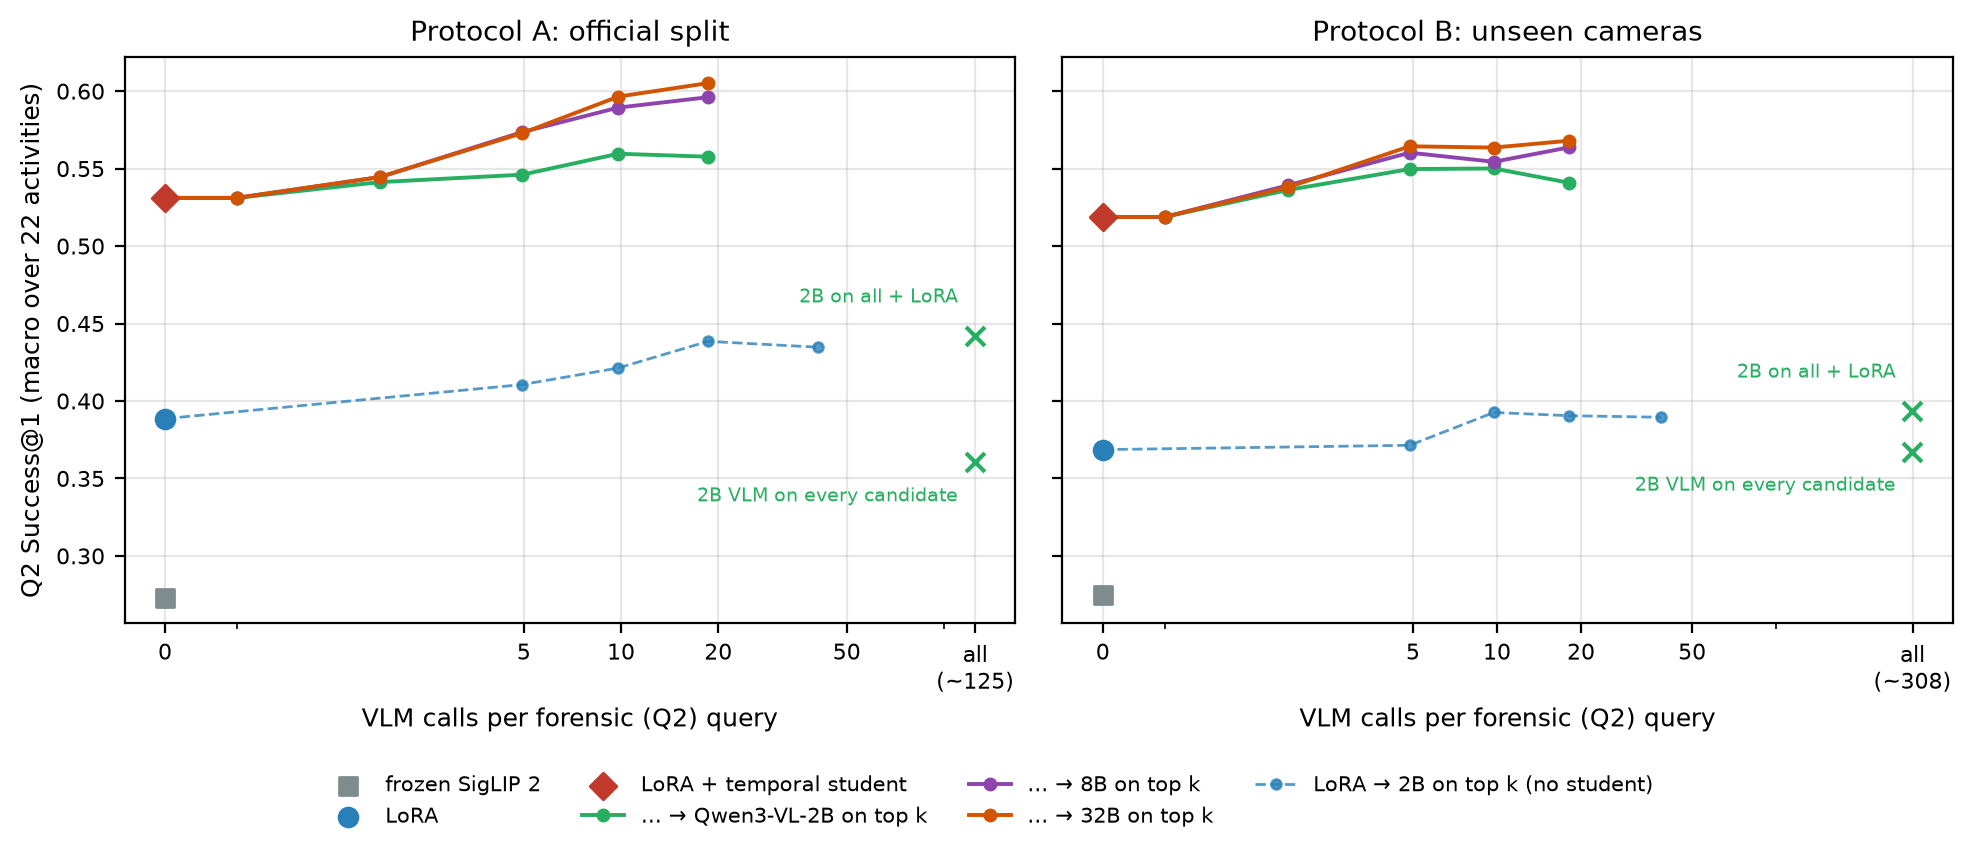
\includegraphics[width=0.82\linewidth]{fig2_cost_curve.png}
\caption[Quality-versus-cost curve (Success@1 against VLM calls).]{Quality-versus-cost curve: forensic Success@1 against VLM calls per query. The temporal transformer at 0
calls captures most of the gain; larger VLMs add to it on a short list; the 2B VLM on every candidate is below
LoRA alone.}\label{fig:cost}
\end{figure}

\subsection{Qualitative Results}
Figure~\ref{fig:example} follows one test clip through the system for the query ``a person picking up an object''.
The frozen encoder ranks the correct clip 286th of 3,726; LoRA moves it to 126th; the temporal transformer, which
sees the person bend down and then straighten up with the item, ranks it first. Figure~\ref{fig:activity} shows the
same effect over all activities: the largest gains of the transformer are on activities defined by motion.

\begin{figure}[H]
\centering
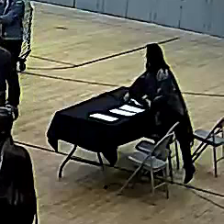
\includegraphics[height=3.0cm]{arch_frame_0.png}\hspace{2pt}
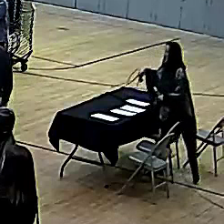
\includegraphics[height=3.0cm]{arch_frame_1.png}\hspace{14pt}
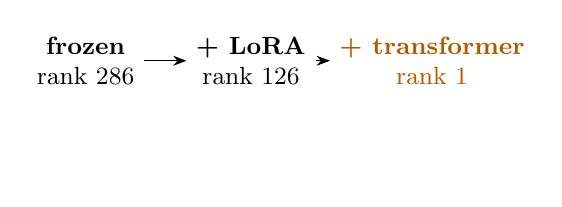
\begin{tikzpicture}[baseline=-1.5cm, font=\small]
\node[align=center] (a) at (0,0) {\textbf{frozen}\\rank 286};
\node[align=center] (b) at (2.1,0) {\textbf{+ LoRA}\\rank 126};
\node[align=center, text=orange!70!black] (c) at (4.4,0) {\textbf{+ transformer}\\rank 1};
\draw[-{Stealth}] (a) -- (b); \draw[-{Stealth}] (b) -- (c);
\end{tikzpicture}
\caption[Sample output: one test clip through the three stages.]{Sample output: two frames (1\,s apart) of MEVA test clip 9850, ``a person picking up an object'', and its rank
among 3,726 test clips at each stage.}\label{fig:example}
\end{figure}

\begin{figure}[H]
\centering
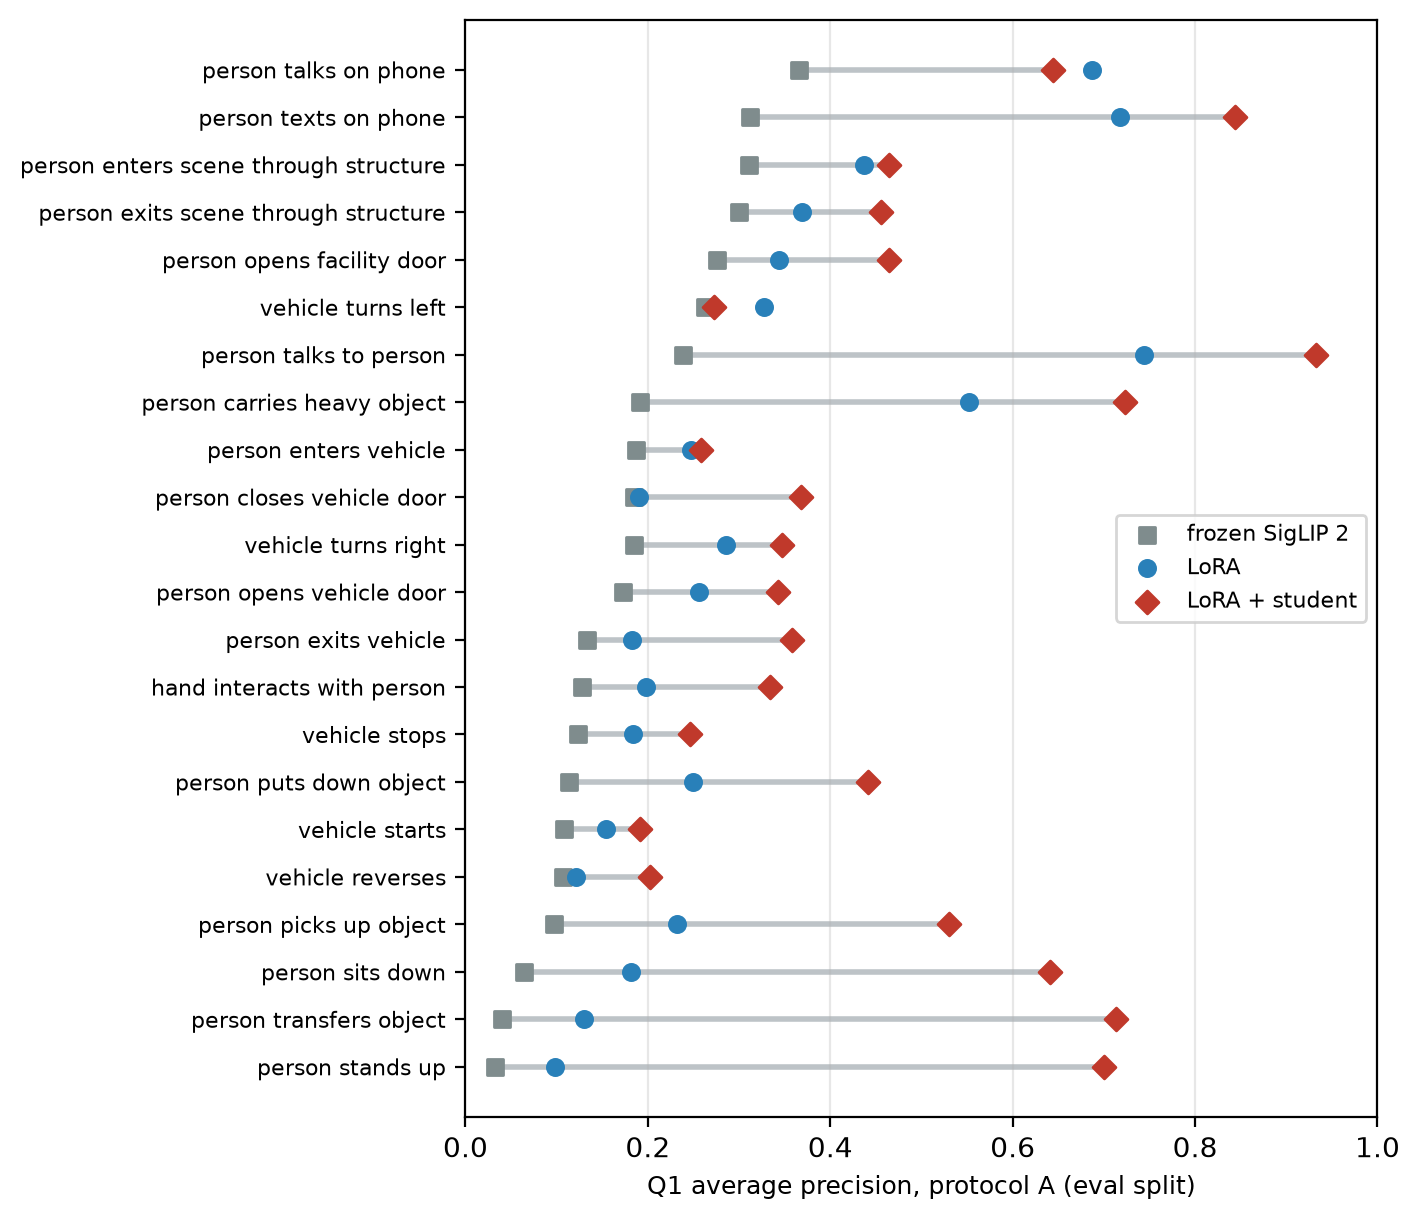
\includegraphics[width=\linewidth]{fig3_per_activity.png}
\caption[Average precision per activity (protocol A).]{Average precision per activity on protocol A (frozen $\rightarrow$ LoRA $\rightarrow$ LoRA + temporal
transformer), sorted by the frozen score.}\label{fig:activity}
\end{figure}

Notable per-activity changes on A: \act{person talks to person} AP 0.238 $\rightarrow$ 0.744 (LoRA) $\rightarrow$
0.932 (transformer); the motion-defined activities (pick up, put down, stand up, transfer an object) from 0.19--0.21
to 0.56--0.57. The search dashboard (Figure~\ref{fig:dash}) answers ``a person opening a car door'' with 6 correct
clips in the top 10 at the Standard level in 0.6\,s, against 4 at the Fast level.

\begin{figure}[H]
\centering
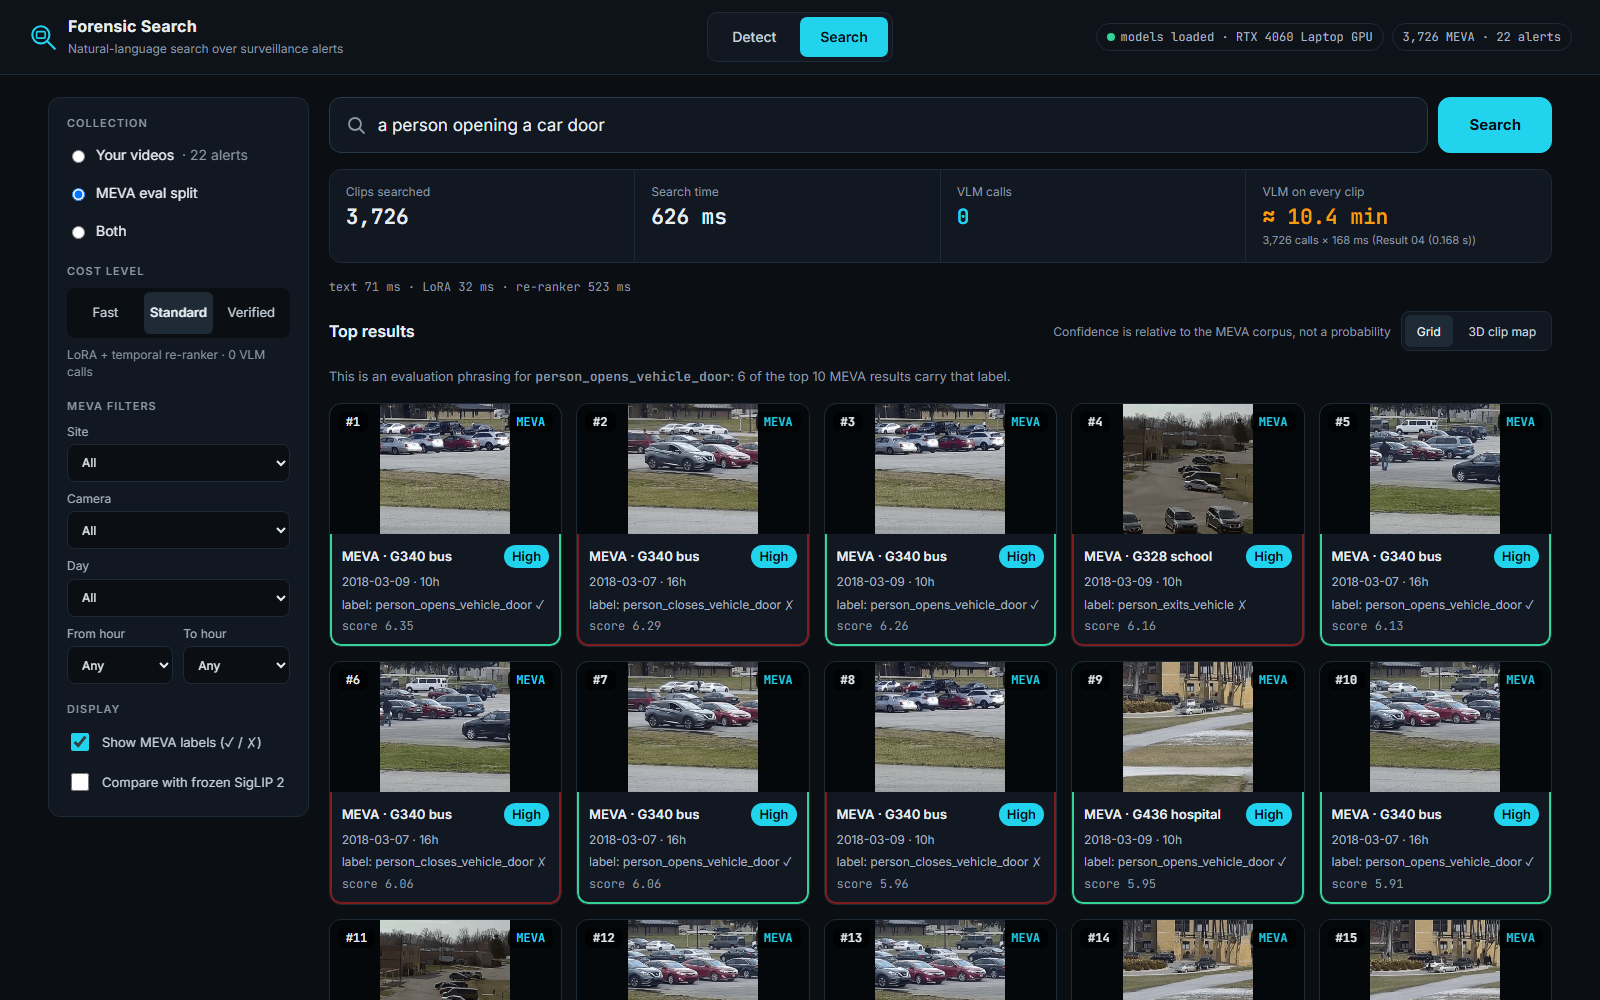
\includegraphics[width=0.95\linewidth]{fig4a_search.png}
\caption[The search dashboard.]{The search dashboard: a test phrasing at the Standard level, correct results marked, with the cost of the
query (0 VLM calls) against a VLM on every clip.}\label{fig:dash}
\end{figure}

\subsection{Ablation Study}
\begin{table}[H]
\centering
\caption[Ablation study.]{Ablations. Validation (val) numbers were used for the choices; test numbers are reported once.}\label{tab:abl}
\small
\begin{tabular}{p{6.6cm}p{3.9cm}p{4.2cm}}
\toprule
\textbf{Change} & \textbf{Result} & \textbf{Conclusion} \\
\midrule
Full frame instead of tight crops (frozen, test A) & Q1 mAP 0.096 vs 0.179 & crop to the actors \\
LoRA frame sampling: middle-weighted vs uniform (test) & A 0.313 vs 0.315; B 0.275 vs 0.280 & no difference \\
Transformer alone, no fusion with LoRA (test A) & S@1 0.460 vs 0.531 & the two scores are complementary \\
Transformer target GT+KD, 2B teacher (val A / B) & 0.594 vs 0.600 / 0.539 vs 0.566 & distillation does not help \\
Transformer target KD only, 2B teacher (val A / B) & 0.424 / 0.377 & teacher weaker than labels \\
Same with the 32B teacher, GT / GT+KD / KD (val A) & 0.606 / 0.573 / 0.447 & still no gain \\
VLM with 16 frames instead of 8 (G1 gain, val) & $+0.006$ / $+0.009$ & more frames do not help \\
LoRA on image + text towers, 2 seeds (val A / B) & $-0.019$ / $+0.047$ & not adopted (rule + drift check) \\
2B VLM on LoRA's top 10, no transformer (test A) & S@1 0.421 vs 0.389 & small; the transformer is worth more \\
\bottomrule
\end{tabular}
\end{table}

Seven VLMs (Qwen3-VL 2B, 2B-Reranker, 8B and 32B; Qwen2.5-VL 3B and 7B; Gemma~4 E4B) were tested with the G1
gate (Table~\ref{tab:gates} in Appendix~\ref{app:more}). Only the 32B passed. Inside the retriever's own top 50, the
VLMs separate right from wrong clips with an AUC of 0.54--0.66, below the adapted retriever's 0.67, which is why
they add little.

% ================================================================ 6
\section{Discussion}\label{sec:disc}
\paragraph{Why it works.} The frozen encoder fails for two reasons, and each trained component fixes one.
\emph{Domain:} SigLIP~2 was trained on web photographs; CCTV shows small, distant, often low-resolution people from
above. A small LoRA on 192 captions moves the image embeddings towards that domain (+75\,\% Q1 mAP), and since the
same activities improve on unseen cameras, this is not camera memorisation. \emph{Time:} per-frame embeddings carry
no motion, so the frozen and adapted encoders are near chance on standing up or picking up. The temporal
transformer sees the frames in order together with how the boxes move, and these activities gain the most.

\paragraph{Why the VLMs disappointed.} The proposal expected a VLM teacher to be the strongest ranker, to be
distilled into a cheap student. Measured on our data, a 2B VLM is a weaker ranker than the adapted encoder: it
sees 8 small frames and answers a yes/no question, while the encoder was adapted to this footage. A teacher that is
less accurate than the labels cannot teach the student more than the labels do, so distillation never helped. The
large VLMs are useful in a different role: as a final check on a short, already good list.

\paragraph{Failure modes.} (1) Left versus right turns: no component separates them (AUC 0.49--0.51), because the
box features are image-plane displacements and heading relative to the camera is not encoded; a merged ``vehicle
turns'' class is found well (AP 0.57--0.62). (2) Footage unlike MEVA (indoor, close-up) is found but rates low
relative to MEVA scores. (3) The best system still misses the right clip at rank 1 for about four forensic queries
in ten, so it is an aid for an investigator, not an automatic decision.

\paragraph{What I learned.} Measuring before building changes the plan: fixing gates and selection rules in advance
turned a failed hypothesis (distillation) into a clear negative result instead of a tuned-up positive one. Cheap,
domain-specific components beat a large general model used everywhere, and cost has to be measured as carefully as
accuracy.

% ================================================================ 7
\section{Conclusion and Future Work}\label{sec:concl}
\subsection{Conclusion}
We built natural-language search over surveillance video on MEVA and measured its quality as a function of VLM
calls. Three findings: (1) adapting the image encoder with LoRA (1.18\,M weights, 192 captions) is the cheapest
large gain and carries over to unseen cameras; (2) a small temporal transformer trained on the human labels is the
largest single step, reaching Q1 mAP 0.476 and Success@1 0.53 at zero VLM calls, while VLM distillation did not
help; (3) VLMs earn their place only at the end, as a check on the top 10, where an 8B or 32B model adds $+0.06$
Success@1. The resulting system answers a query over 3,726 clips in about a quarter of a second on a laptop GPU,
against about 10 minutes for a 2B VLM on every clip, and it runs end to end on new video as a dashboard.

\subsection{Future Work}
\begin{itemize}
  \item Heading-relative motion features (or a calibrated ground plane) to separate left and right turns.
  \item A retention objective so that adapting the text encoder keeps its gain on unseen cameras ($+0.047$) without
        drifting on general language.
  \item Several training seeds for the selected models, and a prompt and frame-layout study for the VLM gate.
  \item Labelled footage from outside MEVA, to measure retrieval on real (unscripted) CCTV and calibrate the
        dashboard's confidence bands.
  \item Temporal localisation inside long videos, and a quantised student for edge deployment.
\end{itemize}

% ================================================================ references
\begin{thebibliography}{99}\small
\bibitem{clip} A.~Radford et al., ``Learning transferable visual models from natural language supervision,'' in \emph{Proc. ICML}, 2021, pp.~8748--8763.
\bibitem{siglip} X.~Zhai, B.~Mustafa, A.~Kolesnikov, and L.~Beyer, ``Sigmoid loss for language image pre-training,'' in \emph{Proc. ICCV}, 2023.
\bibitem{siglip2} M.~Tschannen et al., ``SigLIP 2: Multilingual vision-language encoders with improved semantic understanding, localization, and dense features,'' arXiv:2502.14786, 2025.
\bibitem{qwen3vl} S.~Bai et al. (Qwen Team), ``Qwen3-VL technical report,'' arXiv:2511.21631, 2025.
\bibitem{lora} E.~J.~Hu et al., ``LoRA: Low-rank adaptation of large language models,'' in \emph{Proc. ICLR}, 2022.
\bibitem{hinton} G.~Hinton, O.~Vinyals, and J.~Dean, ``Distilling the knowledge in a neural network,'' arXiv:1503.02531, 2015.
\bibitem{hofstatter} S.~Hofst\"atter, S.~Althammer, M.~Schr\"oder, M.~Sertkan, and A.~Hanbury, ``Improving efficient neural ranking models with cross-architecture knowledge distillation,'' arXiv:2010.02666, 2020.
\bibitem{cascade} L.~Wang, J.~Lin, and D.~Metzler, ``A cascade ranking model for efficient ranked retrieval,'' in \emph{Proc. ACM SIGIR}, 2011, pp.~105--114.
\bibitem{escorcia} V.~Escorcia, M.~Soldan, J.~Sivic, B.~Ghanem, and B.~Russell, ``Temporal localization of moments in video collections with natural language,'' arXiv:1907.12763, 2019.
\bibitem{qvhighlights} J.~Lei, T.~L.~Berg, and M.~Bansal, ``QVHighlights: Detecting moments and highlights in videos via natural language queries,'' in \emph{Proc. NeurIPS}, 2021.
\bibitem{tran} H.-L.~Tran et al., ``Towards efficient and robust moment retrieval system: A unified framework for multi-granularity models and temporal reranking,'' in \emph{Proc. CVPR Workshops}, 2025.
\bibitem{superimage} T.~Nishimura, S.~Nakada, and M.~Kondo, ``Vision-language models learn super images for efficient partially relevant video retrieval,'' arXiv:2312.00414, 2023.
\bibitem{uca} T.~Yuan et al., ``Towards surveillance video-and-language understanding: New dataset, baselines, and challenges,'' in \emph{Proc. CVPR}, 2024.
\bibitem{vadclip} P.~Wu et al., ``VadCLIP: Adapting vision-language models for weakly supervised video anomaly detection,'' in \emph{Proc. AAAI}, 2024.
\bibitem{surveilens} M.~Owais, A.~Siddiqui, A.~Alam, and S.~Ali, ``SurveiLens: Natural language-based moment retrieval for surveillance video analysis,'' IEEE Xplore document 11400480, 2025.
\bibitem{foresea} H.~Park, Y.~Li, et al., ``ForeSea: AI forensic search with multi-modal queries for video surveillance,'' arXiv:2603.22872, 2026.
\bibitem{meva} K.~Corona, K.~Osterdahl, R.~Collins, and A.~Hoogs, ``MEVA: A large-scale multiview, multimodal video dataset for activity detection,'' in \emph{Proc. WACV}, 2021, pp.~1060--1068.
\bibitem{bytetrack} Y.~Zhang et al., ``ByteTrack: Multi-object tracking by associating every detection box,'' in \emph{Proc. ECCV}, 2022.
\bibitem{yolo} G.~Jocher, A.~Chaurasia, and J.~Qiu, ``Ultralytics YOLO (version 8),'' 2023. \url{https://github.com/ultralytics/ultralytics}
\end{thebibliography}

% ================================================================ appendices
\appendix
\section{Code, Models and How to Run the System}\label{app:code}

\subsection{Shared Folder}
The complete code and the trained models are shared here: \textbf{\CodeLink}. The MEVA dataset is not
redistributed (Appendix~\ref{app:repro}).

\begin{table}[H]
\centering
\caption{Contents of the shared folder.}\label{tab:folder}
\small
\begin{tabular}{p{3.6cm}p{9.0cm}r}
\toprule
\textbf{Folder} & \textbf{Contents} & \textbf{Size} \\
\midrule
\texttt{code/} & Python package \texttt{sfs} (training, evaluation, dashboard), built web page, run scripts, Docker files & $<$0.1\,GB \\
\texttt{models/siglip2/} & SigLIP~2 base (image and text encoder), unchanged & 1.4\,GB \\
\texttt{models/lora\_adapter/} & \textbf{trained} LoRA adapter of the image encoder (1.18\,M weights) & $<$0.1\,GB \\
\texttt{models/index/} & \textbf{trained} temporal transformer (\texttt{student.pt}); embeddings of the 3,726 MEVA test clips & 0.3\,GB \\
\texttt{models/yolo/} & YOLOv8m detector for uploaded videos & $<$0.1\,GB \\
\texttt{models/qwen3-vl-2b/} & Qwen3-VL-2B, used only by the Verified level & 4.0\,GB \\
\texttt{test\_videos/}, \texttt{my\_alerts/} & a CCTV test clip, and the same clip already processed (22 alerts) & 0.1\,GB \\
\bottomrule
\end{tabular}
\end{table}

\subsection{Requirements}
\begin{itemize}
  \item Python 3.12 (the package versions are pinned for it).
  \item Recommended: an NVIDIA GPU with at least 8\,GB and a driver that supports CUDA 12.6 (version 560 or newer);
        tested on an RTX 4060 Laptop GPU under Windows 11. Without a GPU the system runs on the processor, more
        slowly and without the Verified level.
  \item About 6\,GB of disk for the Python packages. No internet connection is needed at run time.
\end{itemize}

\subsection{Installation}
Open a terminal in the \texttt{code} folder and create an environment (Windows shown; on Linux use
\texttt{python3.12} and \texttt{. .venv/bin/activate}):
\begin{lstlisting}[language={},numbers=none]
py -3.12 -m venv .venv
.venv\Scripts\activate
python -m pip install --upgrade pip
pip install -r requirements.txt        (without a GPU: requirements-cpu.txt)
\end{lstlisting}

\subsection{Running the Dashboard}
\begin{enumerate}[leftmargin=*]
  \item In the \texttt{code} folder, with the environment active, run \texttt{run.bat} (Windows) or
        \texttt{./run.sh} (Linux). The message ``MEVA media not found \ldots'' is expected: the dataset is not in
        the folder.
  \item Wait for \texttt{open http://127.0.0.1:8000} (about a minute while the models load) and open that address
        in a browser. Stop the server with Ctrl+C; another port: \texttt{run.bat --port 8010}.
  \item \textbf{Detect tab:} upload a video (\texttt{test\_videos/garage\_cctv.mp4} or any MP4, MOV, AVI, MKV or
        WebM). YOLOv8 finds people, vehicles and backpacks; each object present for 0.5\,s becomes an alert with
        a 5-second clip, embedded with the trained models. Processing takes about four times the video's length
        on a laptop GPU. Alerts are kept in \texttt{my\_alerts/}; the test clip is already processed.
  \item \textbf{Search tab:} type what happened, e.g.\ ``a person walking past a parked car'', and choose a level:
        \emph{Fast} (LoRA-tuned SigLIP~2 only), \emph{Standard} (with the temporal transformer; the main result)
        or \emph{Verified} (Standard, then the VLM on the top $k$). The bar under the search shows the time of
        each stage and what a VLM on every clip would have cost; \emph{Map} shows every clip in 3D.
\end{enumerate}
\textbf{Docker (NVIDIA GPU):} in \texttt{code}, create an empty folder \texttt{../meva} and run
\texttt{docker compose up}; the first run builds a 12\,GB image, then the dashboard is at
\texttt{http://127.0.0.1:8000}. The folder's \texttt{README.md} has the full guide and a troubleshooting table.

\subsection{Dataset and Reproducing the Experiments}\label{app:repro}
MEVA is public (CC BY 4.0) at \url{https://mevadata.org}; the videos are on AWS Open Data
(\url{https://registry.opendata.aws/mevadata/}) and the annotations in the MEVA data repository linked from the
site. The experiments run as modules of the \texttt{sfs} package, in this order:
\texttt{sfs.data.manifest} (clip list, protocols A and B) $\rightarrow$ \texttt{sfs.data.extract\_crops} (crop
store) $\rightarrow$ \texttt{sfs.embed.run} (frozen embeddings) $\rightarrow$ \texttt{sfs.train.run} (LoRA)
$\rightarrow$ \texttt{sfs.embed.reembed} $\rightarrow$ \texttt{sfs.rerank.features} and \texttt{sfs.rerank.train}
(temporal transformer) $\rightarrow$ \texttt{sfs.teacher.run} and \texttt{sfs.teacher.gate} (VLMs)
$\rightarrow$ \texttt{sfs.eval.baseline} and \texttt{sfs.eval.cascade\_run} (results). With the derived MEVA
folders \texttt{meva/crops} and \texttt{meva/previews} next to \texttt{code}, the dashboard also searches the
3,726 MEVA test clips.

\subsection{Code Listings}
The two trained models are defined as follows.

\begin{lstlisting}[caption={Temporal transformer (re-ranker), \texttt{sfs/rerank/model.py}.}]
class TemporalReranker(nn.Module):
    def __init__(self, frame_dim, text_dim=768, d=256, layers=2, heads=4, t_max=16, dropout=0.1):
        super().__init__()
        self.frame_in = nn.Sequential(nn.LayerNorm(frame_dim), nn.Linear(frame_dim, d))
        self.query_in = nn.Sequential(nn.LayerNorm(text_dim), nn.Linear(text_dim, d))
        self.pos = nn.Parameter(torch.zeros(t_max, d))
        layer = nn.TransformerEncoderLayer(d, heads, 4 * d, dropout, batch_first=True, norm_first=True)
        self.encoder = nn.TransformerEncoder(layer, layers)
        self.head = nn.Sequential(nn.LayerNorm(d), nn.Linear(d, 1))

    def forward(self, frames, mask, text):
        """frames (B, T, 1548), mask (B, T) True = real frame, text (B, 768) -> logits (B,)"""
        x = self.frame_in(frames) + self.pos[:frames.shape[1]]
        q = self.query_in(text).unsqueeze(1)
        seq = torch.cat([q, x], dim=1)                       # query token first
        pad = torch.cat([torch.zeros_like(mask[:, :1]), ~mask], dim=1)
        out = self.encoder(seq, src_key_padding_mask=pad)
        return self.head(out[:, 0]).squeeze(-1)              # read out at the query token
\end{lstlisting}

\begin{lstlisting}[caption={Label-aware sigmoid loss for the LoRA training, \texttt{sfs/train/loss.py} (Eq.~1).}]
def label_aware_sigmoid_loss(img_emb, cap_emb, labels, logit_scale, logit_bias):
    """img_emb (N, 768), cap_emb (M, 768), labels (N, M): 1 if caption j describes crop i's activity."""
    logits = img_emb @ cap_emb.T * logit_scale.exp() + logit_bias
    target = labels.float()
    return F.binary_cross_entropy_with_logits(logits, target, reduction="sum") / img_emb.shape[0]
\end{lstlisting}

\section{Additional Results}\label{app:more}

\begin{table}[H]
\centering
\caption[VLMs tested as re-rankers (gate G1).]{VLMs tested as re-rankers of the adapted retriever's top 50 (validation). G1 gain = validation Q1 mAP added; pass bar $+0.02$ on one protocol.}\label{tab:gates}
\footnotesize
\setlength{\tabcolsep}{4pt}
\begin{tabular}{lrrrcc}
\toprule
\textbf{VLM} & \textbf{Params} & \textbf{VRAM (GB)} & \textbf{s / call} & \textbf{G1 gain A / B} & \textbf{Verdict} \\
\midrule
Qwen3-VL-2B-Instruct & 2B & 6.1 & 0.17 & $+0.009$ / $+0.002$ & fail \\
Qwen3-VL-Reranker-2B & 2B & 4.4 & 0.16 & $+0.003$ / $+0.012$ & fail (2B teacher) \\
Qwen3-VL-2B, 16 frames & 2B & -- & -- & $+0.006$ / $+0.009$ & fail \\
Gemma 4 E4B-it & 4B eff. & 7.8 & 0.16 & $-0.014$ / $+0.011$ & fail \\
Qwen2.5-VL-3B-Instruct & 3B & 8.5 & 0.12 & $+0.001$ / $+0.004$ & fail \\
Qwen2.5-VL-7B-Instruct (FP8) & 7B & 11.4 & 0.19 & $+0.001$ / $+0.014$ & fail \\
Qwen3-VL-8B-Instruct (FP8) & 8B & 13.0 & 0.13 & $+0.007$ / $+0.019$ & fail by 0.001 \\
Qwen3-VL-32B-Instruct (FP8) & 32B & 12.3 & 1.74 & $+0.017$ / $+0.037$ & \textbf{pass} \\
\bottomrule
\end{tabular}
\end{table}

\begin{table}[H]
\centering
\caption{Hypotheses fixed before the results, and the verdicts.}\label{tab:hyp}
\small
\begin{tabular}{p{7.2cm}p{2.2cm}p{5.2cm}}
\toprule
\textbf{Hypothesis} & \textbf{Verdict} & \textbf{Basis} \\
\midrule
LoRA adaptation beats the frozen encoder & Confirmed & Q1 mAP 0.179 $\rightarrow$ 0.313 (A); all CIs exclude zero \\
A distilled student keeps most of the teacher's quality & Rejected & KD $\ll$ GT; GT+KD $\approx$ GT (2B and 32B teachers) \\
The accuracy-vs-cost curve is strongly concave & Partly & concave after the student (knee at 5--10 calls); flat for the exhaustive 2B VLM \\
The temporal transformer beats LoRA, most on motion activities & Confirmed & motion AP $+0.36$ vs $+0.13$ for the rest \\
Cascade reaches $\ge$90\,\% of the exhaustive VLM at $\le$10\,\% of the calls & Confirmed, trivially & 152\,\% at 4\,\% of the calls (A) \\
\bottomrule
\end{tabular}
\end{table}

\begin{figure}[H]
\centering
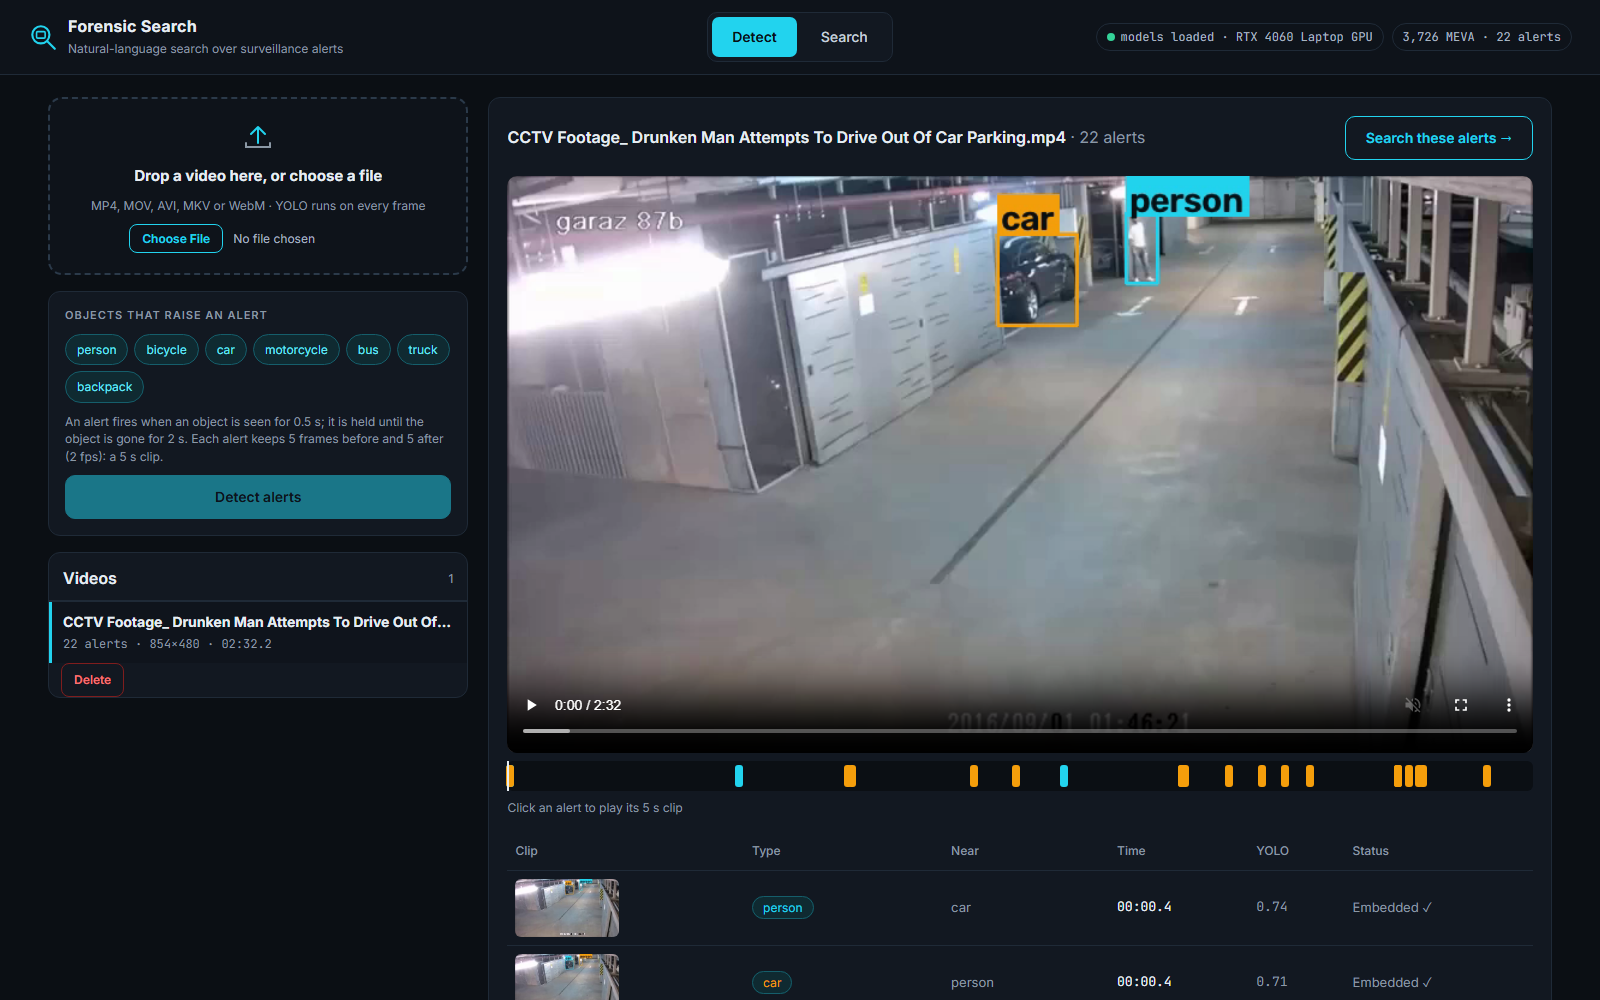
\includegraphics[width=0.49\linewidth]{fig4b_detect.png}\hfill
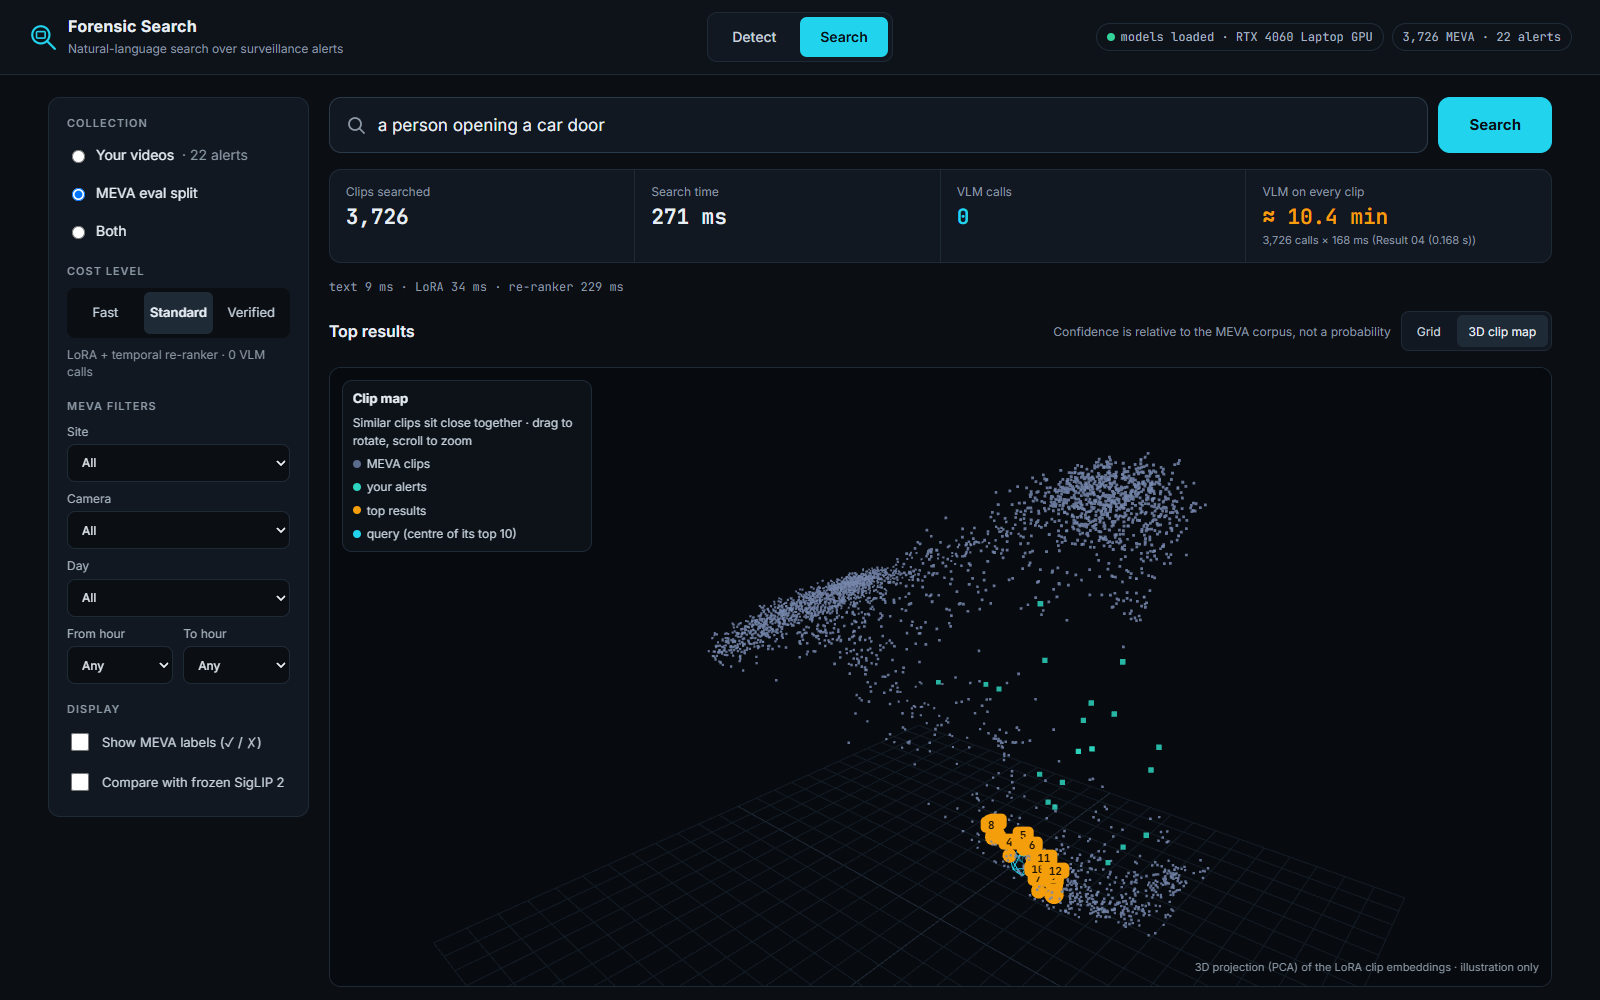
\includegraphics[width=0.49\linewidth]{fig4c_map.png}
\caption[Dashboard on new video: alerts and the clip map.]{Dashboard on new video: alerts detected in an uploaded CCTV clip (left); the 3D map of clip embeddings with
the top results of a query lit up (right).}\label{fig:detect}
\end{figure}

\paragraph{Alerts from new video.} YOLOv8m~\cite{yolo} with ByteTrack~\cite{bytetrack} detects people, vehicles and
backpacks; an object seen for 0.5\,s with confidence $\ge$0.5 raises one alert, held until it has been gone for
2\,s. Each alert keeps a 5-second clip (11 frames at 2\,fps) that goes through the same crops, encoders and
transformer as the MEVA clips, so alerts and MEVA clips share one score scale. A 2.5-minute garage CCTV clip
produced 22 alerts.

\end{document}
